\section{Pattern architetturali}
La \textbf{progettazione architetturale} si occupa dell'organizzazione di un software e della definizione di una sua struttura complessiva; si tratta
del collegamento fra ingegneria dei requisiti e la progettazione, poiché si identificano i componenti strutturali del sistema e le loro relazioni. Il
deliverable è un modello architetturale che descrive in che modo il software è organizzato, in funzione dei suoi componenti.\par
Sono proprio le componenti a identificare le caratteristiche di alto livello del sistema, ragion per cui è data molta importanza alla loro definizione.
Si potrebbe inoltre usare il modello risultante per discutere con gli stakeholder dei progressi fatti.\newline

\noindent In questa fase di sviluppo stiamo assumendo che il documento dei requisiti sia completo e disponibile, perché verrà usato come base per il
design del sistema. Conoscendo "cosa" il software deve fare, adesso dobbiamo definire "come" deve eseguirlo, quindi la \textbf{struttura} della
soluzione, la quale verrà scritta nella fase di implementazione. In particolare, ci sono due livelli di astrazione per la progettazione di architetture
software: \begin{itemize}
	\item \textbf{Alto livello}: Definizione dei macrocomponenti sui quali il sistema verrà architettato.
	\item \textbf{Basso livello}: Definizione delle singole componenti, specificando la soluzione nel dettaglio.
\end{itemize}

\noindent Quello della progettazione è un processo creativo, basato nella maggior parte dei casi sull'adattamento di strutture già conosciute al caso
in esame. Generalmente si fa molto uso degli \textbf{stili architetturali} ad alto livello e dei \textbf{design pattern} a basso livello. La definizione
dell'architettura del sistema ha svariati pregi, come fornire una \textbf{guida} allo sviluppo, semplificando la comprensione del software in ambito di
scelte manageriali e analisi di proprietà. Come conseguenza diretta, il sistema viene documentato e si ha una visione chiara sulla sua evoluzione.\par
Le architetture sono descritte tramite diagrammi a blocchi, i quali presentano una visuale sulla loro struttura e le relative relazioni. Per la
specifica architetturale useremo il linguaggio di modellazione unificato: \textbf{UML}, trattato nelle sezioni successive.\par
Naturalmente, prima di pensare alle componenti è necessario definire la struttura ad alto livello. Già in questa fase è possibile farsi un'idea degli
eventuali costi di sviluppo, in termini di risorse e tempo, con lo scopo di definire un budget più realistico. Ciò fornisce un notevole aiuto durante i
colloqui con gli stakeholder, così che loro possano esprimere le loro preferenze in merito alle caratteristiche del sistema. Il design architetturale,
infatti, impatta principalmente i seguenti campi: \begin{itemize}
	\item \textbf{Prestazioni}: Se lo stakeholder ritiene le performance del sistema la caratteristica più importante, sarà necessario spendere più
	tempo sull'ottimizzazione delle operazioni critiche.
	\item \textbf{Protezione}: Quando la protezione è un requisito critico, è comune utilizzare un'architettura a strati, al cui core sono presenti le
	risorse più importanti.
	\item \textbf{Sicurezza}: Se la sicurezza è importante, bisognerà localizzare le operazioni ad essa relative in un singolo componente o in pochi
	sottosistemi, con lo scopo di ridurre costi e problemi di convalida. Rende inoltre possibile fornire sistemi di protezione che possono bloccare il
	software in caso di guasto.
	\item \textbf{Disponibilità}: Se è richiesto che un sistema debba essere sempre disponibile, bisognerà progettare un'architettura con componenti
	ridondanti e meccanismi per la gestione di guasti, sicché si possa sostituire facilmente la componente problematica e allo stesso tempo mantenere
	il sistema attivo.
	\item \textbf{Mantenibilità}: Se è previsto un software dal lungo ciclo vitale bisognerà renderlo modulare per facilitare il lavoro del team.
	Saranno quindi presenti componenti piccole e con meno dipendenze possibili.
\end{itemize}

\noindent Non esiste il design architetturale perfetto, è necessario scegliere quale modello si adatta al contesto degli stakeholder. Questo perché
alcune architetture presentano conflitti; per esempio, risulta difficile creare un sistema le cui priorità sono prestazioni e protezione, perché, se si
sceglie un design stratificato, per le operazioni critiche sarà presente un notevole overhead in quanto presenti al core, mentre le richieste sono
eseguite al livello più esterno. È quindi verosimile cercare un compromesso tra i vari stili, piuttosto che adattarne uno solo.\par
È quindi estremamente importante conoscere più stili architetturali per semplificare il lavoro di design e banalmente avere più idee riguardo
all'implementazione del software per il dominio applicativo richiesto. Presentiamo quindi gli stili più utilizzati in ambito lavorativo: \begin{itemize}
	\item \textbf{Modello stratificato}: Organizza il sistema in un insieme di livelli; poggia su dei servizi core nascosti agli utenti, sui quali sono
	stratificati i livelli superiori. Ogni livello usa i servizi di quello inferiore e la comunicazione avviene nella maggior parte dei casi tramite
	chiamata a funzione.\par
	Si tratta di un'architettura spesso utilizzata per la scrittura di sistemi operativi. Il vantaggio principale risiede nella sua modifica: se si
	lavora sull'interfaccia di un livello, si influenza esclusivamente quello adiacente, tuttavia, come menzionato prima, è un modello che può risultare
	inefficiente a causa dell'alto numero di chiamate fra i livelli.
	\begin{figure}[h]
		\centering
		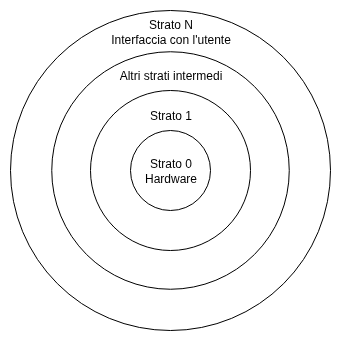
\includegraphics[width=0.5\linewidth]{Images/layered_structure.png}
		\caption{Modello stratificato}	
	\end{figure}
	\item \textbf{Modello repository}: Prevede un componente centralizzato contenente la memoria dei dati e componenti periferici che attuano operazioni
	di lettura e scrittura in questa memoria. Le periferiche non interagiscono tra loro e parlano esclusivamente con la componente centrale. È adatto ad
	applicazioni in cui i dati sono prodotti da un sottosistema e usati da un altro, come i case tool, strumenti che aiutano l'ingegneria del software
	durante il suo ciclo di vita.\par
	Si tratta di un modo efficiente di condividere grandi quantità di dati con una gestione centralizzata del backup e della sicurezza. I sottosistemi
	dovranno tuttavia accordarsi sulla struttura dei dati per il repository; si tratta di un'evoluzione complessa e costosa, che rende difficile
	distribuire il software in maniera efficiente.
	\begin{figure}[h]
		\centering
		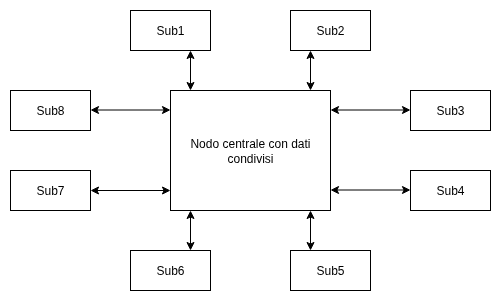
\includegraphics[width=0.8\linewidth]{Images/repository_structure.png}
		\caption{Modello repository}	
	\end{figure}
	\item \textbf{Modello client-server}: Presenta due entità fondamentali; il client, richiedente le informazioni, e il server, che le mantiene e
	fornisce. La comunicazione tra di loro avviene tramite una rete e le periferiche sono fornite da più server che svolgono appositi job a loro
	dedicati.\par
	Si tratta di un modello usato normalmente dalle interfacce dei browser web; spostando la computazione tra i vari server si migliorano le prestazioni,
	il riuso e la mantenibilità. Tuttavia è un sistema distribuito, manca un modello di dati condiviso e il loro scambio può risultare inefficiente per
	questo. Non è semplice gestire il tutto perché possono presentarsi anche delle ridondanze e alcuni server potrebbero essere prorprietari di
	un'azienda, quindi al di fuori del proprio controllo.\par
	Esistono due evoluzioni di questo modello; la prima, \textbf{a due livelli}, presenta tre componenti software di \textbf{interfaccia utente},
	\textbf{gestione dei processi e logica} e \textbf{gestione del database}, distribuiti sui due strati di client e server. La seconda, presenta
	\textbf{tre livelli}: uno di \textbf{presentazione}, un secondo per la \textbf{logica} ed il terzo per la \textbf{gestione dei dati}. Il client
	utilizza esclusivamente l'interfaccia utente, mentre gli altri componenti sono tutti gestiti dal server.
	\begin{figure}[h]
		\centering
		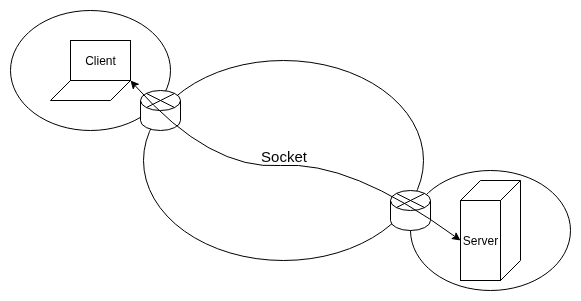
\includegraphics[width=0.8\linewidth]{Images/client-server_structure.png}
		\caption{Modello client-server}	
	\end{figure}
	\item \textbf{Modello peer to peer}: Questa architettura vede ogni componente svolgere il ruolo di client e server mentre esegue il proprio processo.
	Ogni elemento ha infatti un'interfaccia che specifica i servizi offerti. La comunicazione si basa quindi sulla richiesta e offerta dei servizi.\par
	I sistemi p2p scalano bene grazie alla facilità di inserimento dei nodi nuovi e sono tolleranti ai guasti, perché il "perno" sul quale si regge la
	struttura è decentralizzato.
	\item \textbf{Modello pipe and filter}: Presenta due entità fondamentali; i filtri, che effettuano trasformazioni sui dati, e i connettori che lo
	trasmettono ai vari filtri. Si tratta di un sistema che supporta l'esecuzione in parallelo e il riuso delle informazioni. Inoltre, ha un workflow
	intuitivo, rendendo semplice aggiungere e implementare trasformazioni. Tuttavia, non è adatto a software interattivi, ed è infatti usato spesso nello
	sviluppo di sistemi batch. Un esempio di questo sistema è il comando grep della bash UNIX.
\end{itemize}

%

\section{Modelli di controllo}
Per quanto riguarda il design architetturale, sono presenti anche degli \textbf{stili di controllo} del workflow per decidere come gestire il
funzionamento del sistema. Ne esistono due principali: \begin{itemize}
	\item \textbf{Centralizzato}: Un sottosistema ha la responsabilità generale del controllo; avvia e termina gli altri componenti del software.
	\item \textbf{Basato su eventi}: Un sottosistema può rispondere ad eventi generati da altre entità, non esiste quindi un vero e proprio controllore.
\end{itemize}

\noindent L'importanza di conoscere i modelli di controllo risiede nello stesso contesto dei pattern architetturali: la definizione del "come fare" non
è completa se si fornisce esclusivamente una visuale astratta del sistema, ragion per cui andiamo nel dettaglio di come sarà gestito il workflow del
software: \begin{itemize}
	\item \textbf{Modello call-return}: Presuppone l'esistenza di un sottosistema di controllo (\textbf{Main}) che attiva e cede il controllo ad altri
	componenti. Decide inoltre l'ordine di esecuzione e, al termine dell'esecuzione della sottocomponente, riprende il controllo del flusso. Si tratta
	di un modello applicabile esclusivamente a sistemi sequenziali.
	\item \textbf{Modello manager}: Pattern usato quando i sottosistemi possono lavorare in parallelo. Una componente \textbf{manager} controlla avvio,
	terminazione e coordinamento degli altri processi di sistema. Itera continuamente interrogando interfaccia utente, output ed eventuali sensori per
	identificare eventi o cambi di stato. Esempi di questo modello sono i sistemi di allarme; il manager interpella costantemente le sottocomponenti,
	le quali comunicano l'eventuale verificarsi di un dato evento con il segnale acustico.
	\item \textbf{Modello broadcast}: Contrariamente a quanto visto nei precedenti modelli, un componente può annunciare, quindi fare un broadcast,
	l'esecuzione di uno o più eventi. La trasmissione sarà inviata a tutte le altre entità, ognuna capace di gestirlo, e quelle interessate all'ascolto
	eseguiranno la procedura associata all'evento. Per questa ragione, un modello tale è chiamato anche \textbf{event-driven}.\par
	I sistemi di sorveglianza utilizzano questo modello, poiché richiedono una costante allerta per gli eventi, la cui segnalazione deve essere
	comunicata a tutte le apparecchiature in ascolto. È facilmente mantenibile perché risulta semplice aggiungere e rimuovere entità. Tuttavia non è
	sicuro che l'evento venga gestito da una componente; come conseguenza diretta si potrebbero anche perdere dati importanti durante la trasmissione
	non ascoltata.
	\item \textbf{Modello a microservizi}: Approccio per lo sviluppo di una singola applicazione come una suite di piccoli servizi, ognuno eseguito nel
	proprio ambiente e comunicante con gli altri mediante meccanismi semplici, come una API di risorse HTTP. È un modello orientato ai servizi offerti
	dal software nettamente più mantenibile rispetto ai precedenti, poiché le varie componenti hanno dimensioni ridotte e sono indipendenti l'una
	dall'altra. Ogni microservizio realizza una funzionalità, possiede le proprie risorse ed è coordinato con gli altri.\par
	Un'altra caratteristica di questo modello è che le varie componenti possono essere scritte in linguaggi di programmazione diversi, perché sono
	collegati da un gateway\footnote{API Gateway. Si tratta di un design pattern.} per la loro coordinazione.
\end{itemize}
\noindent Arrivati a questa fase del lavoro, si suppone che il design di alto livello, quindi delle specifiche del software e le sue relative interfacce,
abbia avuto un riscontro positivo, consentendoci di andare più nel dettaglio e iniziare la \textbf{scrittura delle componenti}. Si determinano le
specifiche dettagliate scrivendo interfacce dei singoli elementi che compongono il software, quindi i loro campi, metodi e relazioni necessari per
svolgere la propria funzione.\par
Un primo metodo di design per la scrittura di componenti è il \textbf{design by contract}: una progettazione che implementa un \textbf{contratto} tra
due entità, il quale deve specificare gli obblighi di entrambe per garantire il loro corretto funzionamento. Si crea un contratto per ogni componente
del sistema prima che sia codificata ed è composto da più elementi: \begin{itemize}
	\item \textbf{Pre-condizioni}: Espressioni a valori booleani che rappresenta le aspettative sullo stato del programma prima dell'esecuzione di
	un'operazione.
	\item \textbf{Post-condizioni}: Espressioni a valori booleani riguardanti lo stato del software dopo l'esecuzione di un'operazione.
	\item \textbf{Invariante di classe}: Condizione che ogni oggetto della classe deve soddisfare in ogni momento in cui è possibile svolgere
	un'operazione.
\end{itemize}
\noindent Nei contratti si definiscono quindi responsabilità e condizioni da rispettare delle componenti coinvolte; quando queste sono violate, nella
pratica viene lanciata un'eccezione. Si definiscono infatti due entità: un \textbf{client}, il cui compito è garantire la validità delle pre-condizioni,
e un \textbf{fornitore}, che garantisce la correttezza delle post-condizioni in base alla validità di quanto passato dal client.\par
Questa divisione dei compiti ben specificata è molto utile per vari motivi: in primo luogo, facilita notevolmente il \textbf{debugging}, poiché grazie
ai ruoli è possibile ricondursi alla componente che ha lanciato l'eccezione. Se non valgono le pre-condizioni, la colpa sarà del client, mentre se sono
violate le post-condizioni il problema sarà situato nel fornitore. In secondo luogo, guida il team nell'implementazione e mantenimento del software,
perché presuppone una chiara definizione dei compiti nel contratto, semplificando anche la scrittura degli unit test.\par
In generale, scrivere componenti con il metodo design by contract è molto importante, poiché senza una chiara definizione, si potrebbero effettuare
controlli ripetuti delle condizioni in parti diverse del codice, danneggiando le prestazioni con le ridondanze.

%

\section{Principi di progettazione}
Ottenute le specifiche delle singole componenti, si passa alla fase di \textbf{design} delle \textbf{strutture dati} da implementare e
\textbf{algoritmi} da utilizzare. Si tratta di un'attività lasciata in gran parte agli sviluppatori e presenta alcune sottofasi: \begin{enumerate}
	\item Analisi del design della classe da scrivere.
	\item Selezione o definizione dell'algoritmo con la relativa notazione.
	\item Scrittura dell'algoritmo mediante \textbf{step-wise refinement}.
	\item Uso dei metodi formali per dimostrare la correttezza del codice.
\end{enumerate}
\noindent Per la notazione degli algoritmi abbiamo a disposizione diversi strumenti, i quali possono essere \textbf{testuali}, come lo pseudocodice,
oppure \textbf{visuali}, come diagrammi UML. Prendiamo ora un esempio pratico su cui utilizzare lo step-wise refinement: si inizia con la lettura delle
specifiche e si definiscono le dinamiche dell'algoritmo, come i ruoli di client e fornitore insieme ai parametri dei metodi.\par
Dopodiché si passa ad una scrittura più profonda definendo il workflow dei singoli metodi, fino a quando non si è completato l'algoritmo. Lo scopo è
ottenere una forma simile alla seguente: \begin{algorithm}[h]
	\caption{getMax(a, b, c)}
	\begin{algorithmic}[i]
		\Require $a$: int, $b$: int, $c$: int
		\State max $\gets$ calcMax(a, b, c)
		\State min $\gets$ calcMin(a, b, c)
		\State res $\gets max-min$
		\State \textbf{return} res
	\end{algorithmic}
\end{algorithm}

\noindent Quello del design è un processo creativo, ma richiede anche dei \textbf{principi di progettazione} per garantire uno standard e guidare lo
sviluppo verso il raggiungimento di obiettivi di qualità. Ne esistono molteplici e portano a produrre software mantenibile, comprensibile, semplice da
testare, riutilizzabile, portabile e chiaro.\par
Un primo modello è dato dai \textbf{moduli}: entità software identificate da un nome che contiene e fornisce servizi. Presenta un'interfaccia, la parte
esternamente visibile, e la parte interna, composta da strutture dati e il codice. I moduli possono interagire fra loro e includerne altri
(creando dipendenze); per esempio, in un programma C è possibile definire più file header da includere nel codice.\par
Un'altra idea è l'\textbf{astrazione}, la quale consente di concentrarsi su un problema ad un determinato livello senza perdersi in dettagli di quelli
sottostanti. Aiuta a ridurre la complessità e permette di descrivere il comportamento dei moduli più facilmente. Inoltre, nasconde informazioni che gli
altri livelli non devono conoscere. Ne esistono diverse forme: \begin{itemize}
	\item \textbf{Funzionale}: Definisce una funzionalità indipendentemente dall'algoritmo che la implementa.
	\item \textbf{Di dati}: Definisce un tipo di dato in base alle operazioni che si attuano su di esso senza definire una struttura concreta.
	\item \textbf{Di controllo}: Definisce un meccanismo di controllo senza mostrare i dettagli interni.
\end{itemize}
\noindent La terza idea è data dalla \textbf{decomposizione}, quindi la partizione di un problema complesso. Conosciuto anche come Divide-et-Impera,
consente una più semplice gestione dei problemi in quanto di dimensione ridotta. Impiegando questo principio, tuttavia, sarà necessario spendere anche
del tempo per l'integrazione di ogni modulo creato.\par
Una diretta conseguenza della decomposizione è la \textbf{modularità}, un principio che fornisce un criterio detto \textbf{separation of concerns} per
la divisione del software: tenere separati gli aspetti che non si riguardano di un software. È infatti buona prassi mantenere separati in moduli le
componenti di generazione dati (backend) da quelle necessarie alla presentazione (frontend), seguendo una linea guida per massimizzare la coesione e
minimizzare l'accoppiamento. Un modulo si dice \textbf{coeso} se esegue un solo compito e usa le proprie risorse a disposizione, interagendo il meno
possibile con altre entità.\par
L'\textbf{accoppiamento} è invece una metrica per il grado di dipendenza tra i moduli; quando è alto risulta più difficile apportare modifiche alle
entità. Non è realistico avere moduli perfettamente indipendenti, ragion per cui è a discrezione del designer trovare un giusto compromesso.
Generalmente, un buon accoppiamento è dato dalle chiamate di metodi di altri moduli; è inevitabile. Dei flussi evitabili sono invece quelli dove una
componente modifica i dati di un'altra; sarebbe più corretto far gestire a un modulo le proprie risorse, eventualmente \textbf{nascondendole} agli
altri.\par
I modificatori di accesso permettono di implementare il paradigma di \textbf{information hiding}; non tutte le informazioni devono essere pubbliche
all'interno del software e quelle che non sono utili agli altri moduli dovrebbero essere rese private in quelle componenti dove sono necessarie. Se la
tecnica è descritta tramite interfacce si ha come diretta conseguenza la creazione di moduli coesi.\newline

\noindent È possibile rappresentare le dipendenze tramite un grafo; ciò aiuta a comprendere le modalità in cui i moduli sono accoppiati. Diciamo
\textbf{fan-in} quando una dipendenza è entrante, mentre \textbf{fan-out} se è uscente. In particolare, un alto numero di fan-in indica un buon riuso
del modulo in più contesti; al contrario, un alto numero di fan-out mostra un'eccessiva dipendenza e bisogna valutare se decomporre il modulo. Si
richiede di trovare un compromesso.\par
Un'altra proprietà molto importante per i moduli è quella della \textbf{generalità}: impatta principalmente il grado di riutilizzabilità. È buona prassi
cercare di rendere le componenti adattabili a più contesti se si ritiene possano essere utilizzate più volte. Un esempio è dato dagli algoritmi di
ordinamento; se definiti in modo generale è possibile dar loro qualunque input e sapranno riportare un risultato corretto.\par
Infine, è impossibile non menzionare la tecnica \textbf{dry kiss}, ovvero \textbf{don't repeat yourself}, \textbf{keep it simple, stupid}. Bisogna
scrivere codice il meno ripetitivo e quanto più chiaro possibile; se il workflow si "commenta da solo" leggendolo ed è presente una sola volta
all'interno del programma, è stato fatto un buon lavoro.

%

\section{Design Pattern}
I \textbf{pattern di design} sono soluzioni standardizzate per dei problemi specifici di programmazione orientata agli oggetti, le quali costituiscono
anche eventuali unità di riuso. Aiutano ad applicare i principi di buona progettazione, l'implementazione del design architetturale, ma possono anche
essere utilizzati durante la modellazione e la codifica del software, facilitando la comunicazione tra sviluppatori. Altre unità di riuso disponibili
sono \begin{itemize}
	\item \textbf{componenti riusabili} (COTS): Parti di applicazioni di cui è fornita l'interfaccia, ma l'implementazione non è visibile.
	\item \textbf{Framework}: Insieme di classi e interfacce cooperanti che realizzano un design riutilizzabile e adattabile in più domini operativi.
	\item \textbf{Product lines}: Famiglie di prodotti sviluppati da uno stesso nucleo.
	\item \textbf{Librerie}: Insiemi di operazioni riutilizzabili in più contesti.
\end{itemize}

\noindent I design pattern si differenziano da queste unità perché rappresentano un concetto più astratto. Non è possibile applicarli direttamente,
bensì è necessario adattarli al contesto operativo; inoltre, non concernono l'intera architettura del sistema, bensì solo alcune parti dove è ritenuto
opportuno applicarli. Per esempio, in un sistema può capitare di avere la necessità di fornire uno spazio di dati condiviso, rendendo corretta
l'applicazione di \textbf{Singleton}\footnote{Design pattern che garantisce l'esistenza di un solo oggetto della classe in tal modo definita.}, ma ciò
non significa che tutte le classi debbano necessariamente avere un solo oggetto. In ogni caso, i pattern elementari (GRASP) sono usati per
l'assegnazione delle responsabilità nel software e costituiscono il confamento per la progettazione di sistemi orientati agli oggetti. In particolare,
distinguiamo tre sottocategorie: \begin{itemize}
	\item \textbf{Creazionali}: Definiscono modalità di istanziazione degli oggetti, come Abstract Factory.
	\item \textbf{Strutturali}: Definiscono la composizione di classi e oggetti, come Adapter e Facade.
	\item \textbf{Comportamentali}: Definiscono l'interazione tra gli oggetti e distribuiscono le varie responsabilità, come il Template Method, State e
	Observer.
\end{itemize}

\noindent La descrizione di un design pattern presenta una struttura standardizzata, composta di quattro sezioni: il relativo \textbf{nome}, un
\textbf{problema da risolvere}, la \textbf{soluzione} fornita dal pattern e le \textbf{conseguenze} che porta la sua applicazione. Vediamo alcuni
esempi concreti.\newline

\noindent \textbf{Factory}: Design pattern creazionale che fornisce un'interfaccia per la creazione di oggetti in una superclasse, ma consente alle
eventuali sottoclassi di alterare il tipo di oggetti da creare.\par
Supponiamo di avere un sistema per la logistica. Una prima versione gestisce il trasporto solo mediante oggetti \textit{Truck} e il grosso del codice
è scritto al loro interno. Nel caso in cui si abbia la necessità di gestire trasporti con mezzi diversi, tuttavia, sarà necessario apportare modifiche
all'intera codebase, perché la responsabilità non sarà più solo delle classi \textbf{Truck}.\par
La soluzione fornita da Factory suggerisce il rimpiazzo delle instanziazioni dirette degli oggetti, in questo contesto chiamati \textbf{prodotti}, con
invocazioni ad un metodo ad hoc specifico per la loro creazione. Il vantaggio diretto di questo approccio è la possibilità di fare override del metodo
in una sottoclasse ed eventualmente modificare la classe del prodotto da creare.\newline

\noindent Un pattern simile è poi quello della \textbf{Abstract Factory}: pattern creazionale che consente di produrre famiglie di oggetti legati da una
relazione senza specificare le loro classi concrete.\par
Immaginiamo di avere un sistema gestionale per un negozio di vendita di mobili. Il codice presenterà classi di famiglie dei vari prodotti, come
\textit{Chair}, \textit{Sofa} e simili. Queste classi tuttavia presentano delle varianti ed è quindi necessario trovare un modo per creare oggetti
concreti che rispecchino la caratteristica in esame. Inoltre, pensare di cambiare il codice esistente ad ogni nuovo tipo di prodotto è impensabile
poiché estremamente dispendioso in termini di tempo e risorse. La soluzione Abstract Factory si attua in due fasi: \begin{enumerate}
	\item Dichiarazione di interfacce per ogni famiglia distinta di prodotti, quindi una per \textit{Chair}, una per \textit{Sofa}, etc, in tal modo
	che eventuali nuovi prodotti di quell'insieme seguano le stesse dinamiche.
	\item Dichiarazione di una classe \textit{AbstractFactory}, un'interfaccia con una lista di metodi creazionali per ogni prodotto facente parte di
	una determinata famiglia. Queste procedure devono ritornare necessariamente tipi di prodotto \textbf{astratti} rappresentati dalle interfacce
	definite prima. Per ogni variante di prodotto bisognerà creare una classe \textit{Factory} concreta che implementa quella astratta e ritorna il
	prodotto concreto desiderato.
\end{enumerate}

\noindent Il codice dovrà quindi lavorare con le fabbriche e i prodotti mediante le rispettive interfacce astratte. Ciò consente di cambiare il tipo di
fabbrica che viene passato al richiedente, come anche la variante di prodotto che riceve, senza modificare il codice del client.\newline

\noindent Per quanto riguarda i pattern strutturali, il primo degno di nota è \textbf{Adapter}\footnote{Chiamato anche Wrapper.}, il quale consente di
far collaborare due oggetti le cui interfacce sarebbero altrimenti incompatibili.\par
Supponiamo di voler creare un'applicazione per monitorare il mercato azionario, la quale fa un download dei dati da più fonti per esportarlo in formato
XML e mostrarlo in modo pulito con un'apposita interfaccia utente. Dopo un pò, si contempla l'idea di integrare una libreria di terze parti, ma questa
lavora esclusivamente con file JSON.\par
La soluzione di Adapter richiede la creazione di un oggetto speciale che converte le interfacce di un oggetto sicché un altro possa comprenderlo e
collaborarci. Un adattatore nasconde quindi la complessità nativa con un'astrazione comprensibile dall'altra parte, generalmente incurante del fatto
che sia un adattatore.\newline

\noindent Un prossimo pattern strutturale è \textbf{Facade}, che fornisce un'interfaccia semplificata a una libreria, un framework, o più in generale
qualunque altro insieme complesso di classi.\par
Supponiamo di avere la necessità di rendere il codice funzionale con un vasto insieme di oggetti appartenenti a un Framework. La soluzione della
facciata richiede la creazione di un'interfaccia più semplice con funzionalità essenziali dell'intero set di classi. Per esempio, un'applicazione atta
al download di video su YouTube potrebbe usare una libreria contenente anche funzioni di riproduzione dei file. Queste ultime, tuttavia, esulano dallo
scopo del nostro software, e la facciata non le comprenderebbe in quanto tali.\newline

\noindent Passando ai pattern comportamentali vediamo anzitutto il \textbf{Template method}, che definisce lo scheletro di un algoritmo in una classe,
le cui sottoclassi faranno override su step specifici della procedura senza modificarne la struttura intera.\par
Supponiamo di avere un'applicazione per il data mining, il cui scopo è estrarre informazioni dai documenti forniti. La prima versione gestisce solo il
formato DOC, ma nelle successive si migliora il sistema rendendolo capace di lavorare anche sui CSV e PDF. Tuttavia, è evidente che molto codice è
simile o duplicato nelle classi specifiche per formato.\par
La soluzione del template suggerisce di spezzare l'algoritmo in una serie di passi definiti in metodi diversi, ognuno dei quali potrà essere overridato
e reso specifico per il formato desiderato, rimuovendo il codice duplicato in toto.








\begin{comment}
-- Observer
Observer is a behavioral design pattern that lets you define a subscription mechanism to notify multiple objects about any events that happen to the object they’re observing.
Imagine that you have two types of objects: a Customer and a Store. The customer is very interested in a particular brand of product (say, it’s a new model of the iPhone) which should become available in the store very soon.

The customer could visit the store every day and check product availability. But while the product is still en route, most of these trips would be pointless.
On the other hand, the store could send tons of emails (which might be considered spam) to all customers each time a new product becomes available. This would save some customers from endless trips to the store. At the same time, it’d upset other customers who aren’t interested in new products.

It looks like we’ve got a conflict. Either the customer wastes time checking product availability or the store wastes resources notifying the wrong customers.
The object that has some interesting state is often called subject, but since it’s also going to notify other objects about the changes to its state, we’ll call it publisher. All other objects that want to track changes to the publisher’s state are called subscribers.

The Observer pattern suggests that you add a subscription mechanism to the publisher class so individual objects can subscribe to or unsubscribe from a stream of events coming from that publisher. Fear not! Everything isn’t as complicated as it sounds. In reality, this mechanism consists of 1) an array field for storing a list of references to subscriber objects and 2) several public methods which allow adding subscribers to and removing them from that list.
Now, whenever an important event happens to the publisher, it goes over its subscribers and calls the specific notification method on their objects.

Real apps might have dozens of different subscriber classes that are interested in tracking events of the same publisher class. You wouldn’t want to couple the publisher to all of those classes. Besides, you might not even know about some of them beforehand if your publisher class is supposed to be used by other people.

That’s why it’s crucial that all subscribers implement the same interface and that the publisher communicates with them only via that interface. This interface should declare the notification method along with a set of parameters that the publisher can use to pass some contextual data along with the notification.
If your app has several different types of publishers and you want to make your subscribers compatible with all of them, you can go even further and make all publishers follow the same interface. This interface would only need to describe a few subscription methods. The interface would allow subscribers to observe publishers’ states without coupling to their concrete classes.

-- State
State is a behavioral design pattern that lets an object alter its behavior when its internal state changes. It appears as if the object changed its class.
The main idea is that, at any given moment, there’s a finite number of states which a program can be in. Within any unique state, the program behaves differently, and the program can be switched from one state to another instantaneously. However, depending on a current state, the program may or may not switch to certain other states. These switching rules, called transitions, are also finite and predetermined.

You can also apply this approach to objects. Imagine that we have a Document class. A document can be in one of three states: Draft, Moderation and Published. The publish method of the document works a little bit differently in each state:

    In Draft, it moves the document to moderation.
    In Moderation, it makes the document public, but only if the current user is an administrator.
    In Published, it doesn’t do anything at all.

	State machines are usually implemented with lots of conditional statements (if or switch) that select the appropriate behavior depending on the current state of the object. Usually, this “state” is just a set of values of the object’s fields. Even if you’ve never heard about finite-state machines before, you’ve probably implemented a state at least once. Does the following code structure ring a bell?

	The biggest weakness of a state machine based on conditionals reveals itself once we start adding more and more states and state-dependent behaviors to the Document class. Most methods will contain monstrous conditionals that pick the proper behavior of a method according to the current state. Code like this is very difficult to maintain because any change to the transition logic may require changing state conditionals in every method.

The problem tends to get bigger as a project evolves. It’s quite difficult to predict all possible states and transitions at the design stage. Hence, a lean state machine built with a limited set of conditionals can grow into a bloated mess over time.

The State pattern suggests that you create new classes for all possible states of an object and extract all state-specific behaviors into these classes.

Instead of implementing all behaviors on its own, the original object, called context, stores a reference to one of the state objects that represents its current state, and delegates all the state-related work to that object.
To transition the context into another state, replace the active state object with another object that represents that new state. This is possible only if all state classes follow the same interface and the context itself works with these objects through that interface.

This structure may look similar to the Strategy pattern, but there’s one key difference. In the State pattern, the particular states may be aware of each other and initiate transitions from one state to another, whereas strategies almost never know about each other.
\end{comment}